% tune.tex
% 9/5/2013 jichi
\section{Program Transformation}
\label{sec-opt}

After selecting the code regions to optimize,
  we currently manually transform the source code to systematically
 enable the overlapping of computation and communication
through the following steps.
%\begin{enumerate}
%\item Function outlining:
%  we split the code region to optimize into \todo { by the communications in it. --- into what subregions? why outlining ?}
%  The interleaved computation and computation are modularized and outlined into functions.
%\item
%Convert blocking communications if existed to non-blocking communication and blocking wait.
%\item Reorder computation and communication by reordering the outlined functions.
%\item
%  If the same data buffer is reused by all loop iterations,
%  we will double the buffers and use different buffers for consequent loop iterations.
%\item
%  We manually insert \texttt{MPI\_Test} into the outlined computation function, and adjust their frequencies to get the best performance.
%  If there is only one communication in the code region, the insertion of \texttt{MPI\_Test} is indispensable to have speed-up.
%\end{enumerate}

\subsection{Function outlining}
Given a loop to optimize, we
first outline the computation and communication inside the loop into separate functions,
in order to make it easier to replicate and reorder them later into different loop iterations. In particular, we divide the statements at each iteration I of the target loop into the MPI communications at iteration I (Comm(I)),
the computation  (Before(I)) that should run before Comm(I), and the computation (After(I)) to evaluate after Comm(I)
Each group of statements is then outlined into a separate procedure,  with the loop index variables as its function parameters.\footnote{These components can alternatively be simply tagged as Comm(I), Before(I), and After(I) if the optimization were to be fully automated; outlining makes it easy to modify the code manually.}
Take NAS FT in Figure~\ref{fig:ft_loop} as an example.  The loop to optimize is divided into
  $Comm(I)$, the MPI communication at iteration I;
  $Before(I)$, the computation before communication at iteration I;
  and $After(I)$, the computation after communication at iteration I.

\subsection{Converting MPI communications}
Each blocking MPI operation, for example, {\em alltoall} collectives and point-to-point send-receives,
is converted to an equivalent nonblocking communication combined with a blocking wait.
For example,  in Figure~\ref{fig:ft_loop}, the outlined communication function $Comm(I)$,  which invokes $MPI\_Alltoall$ internally, is replaced by $Icomm(I)$ and $Wait(I)$, which are the corresponding nonblocking communication ($MPI\_Ialltoall$) and wait operations converted from $Comm(I)$, respectively.

\subsection{Reordering computation and communication}

After the previous steps, the body of the loop to optimize now contains a sequence of specially
named operations such as
 $Before(I)$, $After(I)$, $Icomm(I)$, and $Wait(I)$,
  where $I$ is the loop index variable looping from $1$ to $N$.
%
% 1:
%   Loop I = 1 .. N
%   - Before(I)
%     Comm(I)
%     After(I)
%
% 2:
%   Loop I = 1 .. N
%   - Before(I)
%     Icomm(I)
%     Wait(I)
%     After(I)
%
% 3:
%   Before(1)
%   Icomm(1)
%   Loop I = 2 .. N
%   - Wait(I - 1)
%     After(I - 1)
%     Before(I)
%     Icomm(I)
%   Wait(N)
%   After(N)
%
% 4:
%   Before(1)
%   Icomm(1)
%   Loop I = 2 .. N
%   - Before(I)
%     Wait(I - 1)
%     Icomm(I)
%     After(I - 1)
%   Wait(N)
%   After(N)
%
We then %\emph{shift}
  \emph{interleave} the communication and computation operations of consecutive loop iterations,
  as illustrated in Figure~\ref{fig:cco:reorder},  in two steps:
\begin{enumerate}
\item Move $Before(1)$ and $Icomm(1)$ to the outside before the first iteration of the loop starts,
  and move $Wait(N)$ and $After(N)$ outside after the last loop iteration
  as shown in Figure~\ref{fig:cco:reorder:c}.
\item Move $Before(I)$ and $Icomm(I)$ above $Wait(I-1)$ and $After(I-1)$
  as shown in Figure~\ref{fig:cco:reorder:d}.
\end{enumerate}
After the reordering, the nonblocking communication in the current iteration I (between $Icomm(I)$ and $Wait(I)$)
   can be processed in parallel with the computation in the previous ($After(I-1)$) and next ($Before(I+1)$) iterations.

\subsection{Replicating the communication buffer}
Each MPI operation needs a dedicated buffer to hold the data being communicated.
Applications typically first allocate the necessary communication buffers at the initialization stage and then reuse
the same buffers in the same MPI operations across different loop iterations.
After applying our optimization, as illustrated in Figure~\ref{fig:cco:shift},
  the communication ($Icomm(i)$ and $Wait(i)$) at each $i$th iteration, where $i \geq 2$,  is overlapped with computation $Before(i+1)$ and $After(i-1)$.
  Assuming that two distinct buffers, {\em InBuf} and {\em OutBuf}, are used for sending and receiving each message, respectively, 
 each buffer needs to be replicated into a pair of equal size to ensure that distinct buffers are used across the overlapping iterations, 
as illustrated in Figure~\ref{fig:cco:dup}.
%In the figure, the $InBuf$ and $OutBuf$ represent the memory of the send/receive data of the communication $Icomm$ shared by all loop iterations.
In particular, we replicate each buffer
  by allocating additional memory outside the loop %that has the same size of the original data buffers
  and then alternately use a distinct buffer in every pair of consecutive loop iterations.
% GWP - do you mean alternately?

%n particular, for each buffer used by $Comm(I)$ that used by the overlapping computation, a new buffer of the same size is created;
%  and then replace the buffers accessed at the odd iteration by the communication
%                   and those accessed at the even iteration by the computation
%  with the replicated buffers.

\subsection{Inserting MPI\_Tests}
% 1. Multi-threaded communication:
% Put computation on one thread, and put communication on the other thread.
% We can explicitly create threads for computation and communication.
% Additionally, the MPI implementation also support implicitly and automatically put the whole background communication onto another thread.
% For example, when we compile MPICH3, there is actually a flag for whether we want to enable this or not. And this threading flag is disabled by default.
%
% When threading exist, there is no need to do MPI_Test to overlap the computation and communication.
%
% 2. Single-threaded communication:
% Put both computation and communication on the thread, which is the typical configuration of MPI.
% In this scenario, to overlap computation with long communication, we need frequently call MPI_Test in the middle of computation to continues poll the MPI communication engine.
%
% However, if the communication itself takes very short time, then calling MP_Test might have no impact and could slowdown the overall performance.

When using nonblocking MPI operations, some CPU time needs to be allocated, by embedding $MPI\_Test$ calls in the local computation,
to ensure continuous progress of the communications.
If the local computation is not inside a loop, we insert one or more $MPI\_Test$ calls evenly distributed into the computation.
%And if insertion of $MPI\_Test$ cause slowdown, it will be removed instead.
On the other hand, if the local computation is inside a loop,
  we insert $MPI\_Test$ into the beginning of the loop body and use a conditional variable to adjust its frequency.
The inserted code is illustrated in Figure~\ref{fig:cco:test}.
In both cases, the frequency of $MPI\_Test$ is empirically adjusted as the application is ported to each architecture.


% https://en.wikibooks.org/wiki/LaTeX/Floats,_Figures_and_Captions
\begin{figure}
{\scriptsize
  \centering
  \begin{subfigure}[b]{.25\textwidth}
\begin{verbatim}
DO I = 1 .. N
  Before(I)
  Comm(I)
  After(I)
END DO
\end{verbatim}
    \caption{Input loop}
    \label{fig:cco:reorder:a}
    \vspace{.1in}
  \end{subfigure}%
  \begin{subfigure}[b]{.25\textwidth}
\begin{verbatim}
DO I = 1 .. N
  Before(I)
  Icomm(I)
  Wait(I)
  After(I)
END DO
\end{verbatim}
    \caption{Decouple blocking comm}%unication
    \label{fig:cco:reorder:b}
    \vspace{.1in}
  \end{subfigure}
  \begin{subfigure}[b]{.25\textwidth}
\begin{verbatim}
Before(1)
Icomm(1)
DO I = 2 .. N
  Wait(I - 1)
  After(I - 1)
  Before(I)
  Icomm(I)
END DO
Wait(N)
After(N)
\end{verbatim}
    \caption{Move first and last iterations}
    %\caption{Loop with iterative computation and communication}
    \label{fig:cco:reorder:c}
  \end{subfigure}%
  %add desired spacing between images, e. g. ~, \quad, \qquad, \hfill etc.
  %(or a blank line to force the subfigure onto a new line)
  \begin{subfigure}[b]{.25\textwidth}
\begin{verbatim}
Before(1)
Icomm(1)
DO I = 2 .. N
  Before(I)
  Wait(I - 1)
  Icomm(I)
  After(I - 1)
END DO
Wait(N)
After(N)
\end{verbatim}
    \caption{Interleave consequent iterations}
    %\caption{Decouple and overlap the communication of the i-th iteration with the computation of the (i-1)-th and (i+1)-th iterations}
    \label{fig:cco:reorder:d}
  \end{subfigure}
\caption{Steps to reorder outlined communication and computation functions}
\label{fig:cco:reorder}
}%\scriptsize
\end{figure}

\begin{figure}
{\scriptsize
  \centering
  \begin{subfigure}[b]{.20\textwidth}
\begin{verbatim}
Before(1, InBuf)
Icomm(1, InBuf)
DO I = 2 .. N
  Before(I, InBuf)
  Wait(I - 1)
  Icomm(I, InBuf
         , OutBuf)
  After(I - 1, OutBuf)
END DO
Wait(N, OutBuf)
After(N, OutBuf)
\end{verbatim}
    \caption{Original communication that uses the same input and output $Buf$}
    \label{fig:cco:dup:a}
  \end{subfigure}%
  \hspace{.01in}
  \begin{subfigure}[b]{.28\textwidth}
\begin{verbatim}
Before(1, InBuf)
Icomm(1, InBuf)
DO I = 2 .. N
  Before(I, I % 2 ==  1 ? InBuf : InBuf2)
  Wait(I - 1)
  Icomm(I, I % 2 ==  0 ? InBuf : InBuf2
         , I % 2 ==  0 ? OutBuf : OutBuf2)
  After(I - 1, , I % 2 ==  1 ? InBuf : InBuf2)
END DO
Wait(N, N % 2 == 1 ? OutBuf : OutBuf2)
After(N, N % 2 == 1 ? OutBuf : OutBuf2)
\end{verbatim}
    \caption{Replicate $Buff$ with $Buff2$ of the same size}
    \label{fig:cco:dup:b}
  \end{subfigure}
\caption{Replicate communication buffers for nonblocking communication}
\label{fig:cco:dup}
}%\scriptsize
\end{figure}

\begin{figure}[h]
{\scriptsize
\begin{verbatim}
DO I = 1 ... L
  If I % Freq == 0
    MPI_Test
  Original_computation_statements
END DO
\end{verbatim}
}%\scriptsize
\caption{Insert MPI\_Test into the hot computation loop at specific frequency $Freq$}
\label{fig:cco:test}
\end{figure}

\begin{figure}[h]
\centering
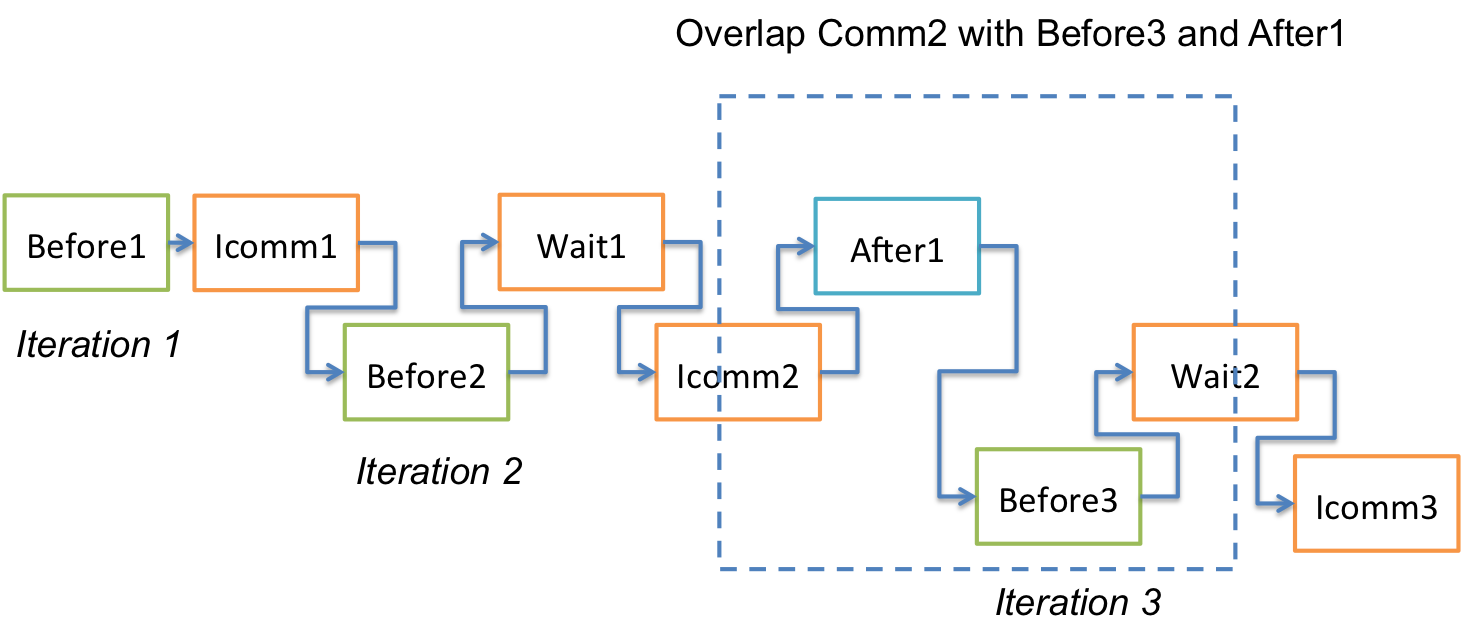
\includegraphics[width=0.49\textwidth]{fig/ft_shift.png} % half page
\caption{Overlapped computation and communication operations}
\label{fig:cco:shift}
\end{figure}

%We insert MPI\_Test into four out of all eight NAS benchmarks.

% EOF

%\begin{figure}
%\centering
%{\scriptsize
%  \begin{subfigure}[b]{0.2\textwidth}
%\begin{verbatim}
%MPI_Ialltoall
%Loop I = 1 ... L
%  If I % Freq == 0
%    MPI_Test
%  Computation
%MPI_Wait
%\end{verbatim}
%  \caption{Single computation loop}
%  \label{fig:cco_test:single}
%  \end{subfigure}%
%  \begin{subfigure}[b]{0.3\textwidth}
%\begin{verbatim}
%MPI_Ialltoall
%Loop I = 1 ... L1
%  If I % Freq1 == 0
%    MPI_Test
%  Computation1
%Loop I = 1 ... L2
%  If I % Freq2 == 0
%    MPI_Test
%  Computation2
%...
%Loop I = 1 ... LN
%  If I % FreqN == 0
%    MPI_Test
%  ComputationN
%MPI_Wait
%\end{verbatim}
%  \caption{Multiple computation loops}
%  \label{fig:cco_test:multiple}
%  \end{subfigure}%
%\caption{Single or multiple computation loops with MPI\_Test inserted}
%\label{fig:cco_test}
%}%\scriptsize
%\end{figure}
%If MPI\_Test is in loops,
%  a condition will be inserted before the MPI\_Test as shown in Figure~\ref{fig:cco_test}
%  to control how many MPI\_Test to execute in the loops, or the \emph{frequency} of MPI\_Test.
%When there are multiple computation loops to insert MPI\_Test,
%  multiple frequencies are needed to be inserted.
%Our experiment results show
%  when MPI\_Test is evenly distributed in the computation time,
%  it can achieve the best performance.
%To make the computation statements in between each pair of MPI\_Test to have roughly equal computation time,
%  the MPI\_Test frequencies are determined by the estimated computation time for loops using analytical modeling
%  so that given two loops L1 and L2:
%\begin{equation}
%  time(Computation_1) * Freq_1 = time(Computation_2) * Freq_2
%\end{equation}
%Given the above relation, the frequencies of multiple MPI\_Test can be control by a single frequency,
%  which is then tuned using binary search on the target runtime environment,
%  i.e. the frequency is constantly increased/decreased when the total execution time is reduced.

%All the point-to-point (send and receive) and collective communication (broadcast, reduce, allreduce, alltoall)
%  being considered in the MPI standards have both blocking and non-blocking functions.
%A blocking function (such as \texttt{MPI\_Alltoall}) can be replaced by a non-blocking function (such as \texttt{MPI\_Ialltoal})
%  and a wait (\texttt{MPI\_Wait}).
%Because \texttt{MPI\_Request} used to connect the non-blocking function and wait
%5  will also be needed by \texttt{MPI\_Test},
%  is is made as a global variable to make it easier to pass to MPI\_Test.
%After decoupling blocking communication, the $Comm$ function will be replaced by $Icomm$ and $Wait$ as shown in Figure~\ref{fig:ft_cco}.

%The variables in the optimization configuration that might carry loop-carried dependence
%  are privatized for each loop iteration.
%If the variables are used as output,
%  the value of the privatized variables are copied to the output variables at the end of each loop iteration.

%To insert the computation in between the decoupled communication,
%  the outlined/specialized computation and communication functions will be reordered
%     as shown in Figure~\ref{fig:ft_cco}.

%Taking the estimated overlap code region by analytical modeling,
%the goal of the CCO analysis stage
%  is to find the computation statements that can be potentially overlapped with the communication.
%There are two ways to overlap the communication and computation.
%The first is to move the computation into the middle of the communication region,
%and (2) interweave the communication and communication loops if both of them are in loops.
%The first one requires the computation that can be safely reordered with the communication;
%and the second one need the computation and communication loops to be fusible.
%Correspondingly, the target computation statements can be divided into two categorized
%  based on their dependence relation to the communication to overlap:
%\begin{enumerate}
%\item Independent computation statements, which are independent from the communication to overlap.
%These statements are able to be reordered freely with the communication in the later program transformation stages.
%\item Decomposable computation loops, which can be safely merged with the communication loops.
%Although there dependence edges between the computation and the communication,
%but after loop fusion, there are no loop carried dependence between communication and communication in the result code.
%As the result, the communication loops and communication can be possibly interwoven.
%\end{enumerate}
%In order to be able to overlap the computation with the communication,
%the computation statements are needed to be \emph{surrounding} with the communication
%that for reach computation statement,
%there is a runtime code path between the computation and a communication
%where all statements on the code path are either independent or decomposable statements.
%%The independent and decomposable workflow is a list of statements
%%  that are either independent from all communication,
%%  or can be decomposable in the same way as the group of communication.
%
%The following subsections will first
%describe the rules to determine independent and decomposable statements,
%then discuss the algorithm to find them in the specified overlap code region.


%The data dependence between a communication and a computation statement
%  is a situation in which one statement refers to the data of the other preceding statement.
%This relation can be determined by analyzing the memory side effects of the statements.

%\subsection{Computing independent and decomposable workflow}

%\subsection{Independent computation}
%An independent computation statement in the overlap code region
%is independent from all communication in the region,
%which means that
%for each communication in the code region,
%there are neither direct nor transitive dependence between the communication and the independent computation.
%The relation could be formally stated as that
%given a independent communication statement $A$ and overlap region $R$,
% independent if for each communication statement $B$ in $R$,
%  there are neither direct nor transitive dependence edge between $A$ and $B$.

%Given this definition, the independent statement can be computed using data dependence analysis.
% Independent condition
%Given a computation and a communication,
%  if there is data dependence between them,
%  they must be both decomposable to loops in order to overlap them.
%
%Assume the computation statement is decomposable to loop $L_1$,
%  and loop $L_2$ is one of the loops that the communication can be decomposed to.
%If loop $L_1$ and $L_2$ can be fused,
%  then the computation and communication are compatible and able to be overlapped after the decomposition.
%
%The communication group could be either a single collective communication,
%  or a list of decoupled send/receive and blocking/non-blocking communication.
%The communication group can be decomposed if the communication statements in the group
%  can be transformed into a loop.

% Communication decomposition
%The CCO analysis stage will select the optimization configurations to apply
%  and the configurations into source code as \emph{CCO annotations}.
%The analysis takes the source code,
%   application's code skeleton,
%   and the hardware performance model as input.
%The optimization configurations include
%  the decomposition patterns for the communication
%  and the functions needed to inline.
%The overall workflow is illustrated in the Figure~\ref{alg:analysis}.


%\subsection{Computing overlappable computation}
%
%The overlappable computation is either
%statements that are independent from the communication,
%or the loops that are fusible with he communication loops.
%Additionally, the computation must be \texttt{reachable} by the communication
%that there is a runtime code path between the computation and the communication
%where all statements on the code path are either independent or decomposable statements.
%Given these requirements,
%  the overlappable computation can be computed using the data-flow analysis and control flow analysis
%  by the following two stepts:
%\begin{itemize}
%\item First, find the first and the last communication in the code region.
%\item Then, traverse the control flow for each statement before the first or after the last communication.
%  If the statement is either independent from or decomposable to the communication,
%  then identify it as overlappable; otherwise stop the traversal.
%\end{itemize}

%Additionally, the compatible computation loop must be \textbf{reachable} by the communication in order to overlap them.
%Given a computation loop $L$ that is compatible with the decomposable communication group $G$.
%In order to overlap them, there must be a list of statements $F$ in the control flow between them
%  where all the statements are in the same code block, or can be moved into the same code block.
%And the statement list $F$ must satisfy one of the following conditions:
%\begin{enumerate}
%\item All statements in $F$ are independent from $G$.
%\item All statements in $F$ are loops that are compatible with $G$.
%\item $F$ can be partitioned into two sub lists.
%The list connecting $G$ are independent from $G$.
%The other list connecting $L$ are loops that are compatible with $G$.
%\end{enumerate}
%The statement list $F$ can be computed in the way similar to that to find the overlap scope stage.
%We can traverse in the overlap code region from $G$ to compute $F$.
%First, if the parent blocks of $G$ are simple blocks that are not loops, branches, and functions,
%  the block boundaries can be eliminated by merging the parent blocks.
%Then, the parent block of $G$ can be divided into two statement lists:
%  one before $G$ and one after $G$.
%Because there are no function calls in the code region after annotation-based inlining,
%  the block of procedure boundary are not needed to be considered.
%% Group of independent statements
%% reachability
%If the group is a list of decoupled communication statements,
%  it can be decomposed if the communication statements are in the same loop.
%If the group is a collective communication,
%  it can be decomposed if the collective communication can be divided into a loop of point-to-point communication.
%There could be different possible ways to decompose a collective communication
%  depending on the portion of data and message size assigned to each point-to-point communication.
%
%The independent and decomposable workflow is a list of statements
%  that are either independent from all communication,
%  or can be decomposable in the same way as the group of communication.
%
%The data dependence between a communication and a computation statement
%  is a situation in which one statement refers to the data of the other preceding statement.
%This relation can be determined by analyzing the memory side effects of the statements.

%A computation statement can be decomposed if it is a loop, or can be transformed into a loop.
%Depending on where the loop is, it can be categorized into the following scenario:
%\begin{itemize}
%\item The statement is a loop.
%\item The loop is in the statement generated by function alls.
%\end{itemize}
%To describe the data access of the decomposed loop,
%  the decomposition can be described as a tuple of
%  $(I, D, P)$ where
%  $I$ is the loop iteration,
%  $D$ is the data accesses per iteration with loop-carried dependence,
%  and $P$ is the  data accesses per iteration without loop-carried dependence.
%Similar to the computation decomposition,
%  the communication decomposition can also be described as the tuple of $(I,D,P)$ for the decomposed loop.
%The difference is that if the communication group is a collective communication,
%  then $D = \emptyset$,
%  and there could be multiple possible $(I,P)$ combinations that could become a decomposition space.
%So, the ways to decompose collective communication could be described as $\{(I,P)\}$, a set of all possible $(I,P)$.
%Given a computation statement $X$ decomposable to $(I,D,P)$,
%and a communication group $Y$ that can be possibly decomposed to any of $\{(I_i,D_i,P_i)\}$,
%then $X$ and $Y$ are compatible if $(I,D,P)$ and any $(I_i,D_i,P_i)$ satisfy any of the following requirements
%(let $W(D)$ represents the write data accesses in $D$):
%\begin{itemize}
%\item $I = I_i$ and $W(D) \cap (D_i \cup P_i) = \emptyset$ and $W(D_i) \cap (D \cup P) = \emptyset$
%\item $I \% I_i = 0$ and $W(D_{tile}) \cap (D_i \cup P_i) = \emptyset$ and $W(D_i) \cap (D_{tile} \cup P_{tile}) = \emptyset$,
%  where $D_{tile}$ and $P_{tile}$ are $D$ and $P$ tiled by $I/I_i$.
%\end{itemize}
%The formal definitions for the reachability is as follows.
%
%Let $C$ be the set of communication statements to overlap.
%Let $S$ be the decomposable communication code represented by a \texttt{BET} statement which is defined as follows:
%\begin{itemize}
%\item If $C$ contains only one collective communication $X$, let $S$ be $X$.
%\item Else if all communication in $C$ are in the same loop $X$, let $S$ be $X$.
%\item Otherwise, the communication cannot be decomposed for overlapping, and $S$ does not exist.
%\end{itemize}
%Let $R$ be the set of statements in the overlap code region.
%Let $I$ be the set of an independent statements to compute.
%A recursive definition of $I$ is as follows:
%\begin{itemize}
%\item Let $X$ be any communication statement in $C$.
%  For each sibling node $Y$ of $X$ in $R$, if $Y$ is independent of $X$, add $Y$ to $I$.
%\item Let $X$ be any communication statement in $C$, and $Z$ be any node in $I$.
%  For each sibling node $Y$ of $Z$ in $R$, if $Y$ is independent of $X$, add $Y$ to $I$.
%\item If $S$ exists, for each sibling node $Y$ of $S$ in $R$, if $Y$ is independent of $S$, add $Y$ to $I$.
%\end{itemize}
%Let $D$ be the set of decomposable statement to compute.
%If $S$ does not exist, which means the communication can not be decomposed, then $D$ is empty.
%Otherwise if $S$ exists, a recursive definition of $D$ is as follows:
%\begin{itemize}
%\item For each sibling node $Y$ of $S$ in $R$, if $Y$ can be decomposed in the same way of $S$, add $Y$ to $D$.
%\item Let $X$ be any decomposable statement in $D$.
%  For each sibling node $Y$ of $X$ in $R$, if $Y$ can be decomposed in the same way of $S$, add $Y$ to $D$.
%\item Let $X$ be any independent statement in $I$ that is outside of $S$.
%  For each sibling node $Y$ of $X$ in $R$, if $Y$ can be decomposed in the same way of $S$, add $Y$ to $D$.
%\end{itemize}
%
%Given two statements $S_2$ and $S_2$.
%Let notation $R(S)$ be the set of data that statement $S$ could read.
%Let notation $W(S)$ be the set of data that statement $S$ could write.
%The relations of the independence and decomposition between two single statements are defined as follows:
%\begin{itemize}
%\item Independence:
%  $S_1$ and $S_2$ are independent if:
%  $R(S_1) \cap W(S_2) = \emptyset \wedge W(S_1) \cap R(S_2) = \emptyset \wedge W(S_1) \cap W(S_2) = \emptyset$.
%\item Decomposition:
%  Let $D = (R(S_1) \cap W(S_2)) \cup (W(S_1) \cap R(S_2)) \cup (W(S_1) \cap W(S_2))$ be the shared data access between the two statements.
%  $S_1$ and $S_2$ can be decomposed in the same way if they satisfy the following requiremens:
%    \begin{enumerate}
%    \item $D \ne \emptyset$
%    \item $S_1$ can be decomposed into a loop. Let $D_1(i)$ be the data in $D$ accessed by the loop body at iteration $i$.
%    \item $S_2$ can be decomposed into a loop. Let $D_2(i)$ be the data in $D$ accessed by the loop body at iteration $i$.
%    \item For any two loop iterations $i$ and $j$: $D_1(i) \cap D_1(j) = \emptyset$.
%    \item For any two loop iterations $i$ and $j$: $D_2(i) \cap D_2(j) = \emptyset$.
%    \item For any loop iteration $i$: $D_1(i) = D_2(i)$.
%    \end{enumerate}
%\end{itemize}


%The problem to decompose the computation and communication in the way that they can be overlapped
%  could be divided into three sub-problems.
%\begin{enumerate}
%\item If it is possible and how to decompose a computation statement
%\item If it is possible and how to decompose the communication group
%\item If it is possible and how to overlap a decomposed computation and communication
%\end{enumerate}
%
%For a computation statement, if it is a loop, it has been decomposed.
%For a collective communication statement, it can be decomposed into a loop of point-to-point communication.
%For a group of point-to-point communication, if their enclosing block is a loop, they has been decomposed.
%
%Given a decomposable computation statement and a decomposable communication group,
%  they can be overlapped if their decomposed loops can be fused.
%Let $L_1$ and $L_2$ be the two decompose loops.
%Let $D$ be the set of data that $L_1$ depends on $L_2$.
%Then, $L_1$ and $L_2$ can be fused if they satisfy the following requirements.
%\begin{enumerate}
%\item There is no loop-carried dependence of $D$ in both $L_1$ and $L_2$.
%\item The data access of $D$ in $L_1$ is equals to or a subset of that in $L_2$'s body.
%\end{enumerate}
%
%
%The output of the independent workflow could be represented by a set of statements
%  where all statements in the set are independent from all communication.
%The output of the decomposable workflow could be represented by a set of statements
%  where all statements in the set can be decomposed together with the communication group in the same way.
%Formal definitions of the concepts are as follows.
%
%The purpose is to compute the computation that are either independent from the communication, or can be decomposed in the same way as the communication.
%There must be on an execution flow $F$ between the communication $A$ and the computation $B$,
%% all statements \textbf{can be transformed into the same block}.
%which satisfies one of the following conditions:
%\begin{itemize}
%\item All statements in $F$ (including $B$) are independent from $A$
%\item There is a statement $S$ in $F$ that can cut $F$ into two segments that all statements between $A$ and $S$ (including $S$) are independent from $A$, and all statements between $S$ and $B$ (including $B$) can be decomposed in the same way as $A$.
%  %or grouped together at the end of the independent execution flow.
%\end{itemize}
%
%\begin{itemize}
%\item Input from within the framework
%  \begin{itemize}
%  \item The overlap region
%  \item Dependence graph for the overlap region
%  \item The communication group to overlap
%  \end{itemize}
%\item Output: Reachable independent and decomposable computation and communication which can be overlapped later
%\end{itemize}
%An example from NAS FT about the reachable path for decomposable statements are as follows.
%The path connecting the decomposable Alltoall communication with the computation is as follows:
%\begin{equation}
%cffts1 \Rightarrow transpose\_xy\_z \Rightarrow transpose2\_local \Rightarrow transpose2\_global
%\end{equation}
%
%{\scriptsize
%\begin{verbatim}
%subroutine FT
%  if (layout_type .eq. layout_1d) then // This is the overlap region
%    call cffts1(1, dims(1,1), dims(2,1), dims(3,1), // Level = 0, inline
%>               x1, x1, scratch)
%    call transpose_xy_z(2, 3, x1, x2)    // Level = 0, inline
%    call cffts2(1, dims(1,3), dims(2,3), dims(3,3),
%>               x2, x2, scratch)
%
%subroutine cffts1(is, d1, d2, d3, x, xout, y) // Level = 0, inline
%  // Decomposable computation hot spot
%  do k = 1, d3
%     do jj = 0, d2 - fftblock, fftblock
%        do j = 1, fftblock
%           do i = 1, d1
%              y(j,i,1) = x(i,j+jj,k)
%           enddo
%        enddo
%        call cfftz (is, logd1, d1, y, y(1,1,2))
%        do j = 1, fftblock
%           do i = 1, d1
%              xout(i,j+jj,k) = y(j,i,1)
%           enddo
%        enddo
%     enddo
%  enddo
%  return
%  end
%
%subroutine transpose_xy_z(l1, l2, xin, xout) // Level = 0, inline
%  call transpose2_local(dims(1l1)*dims(2,l1),dims(3,l1), // Decomposable
%> xin,xout)
%  call transpose2_global(xout,xin) // Decomposable communication
%  call transpose2_finish(dims(1,l1)*dims(2,l1),dims(3,l1)
%> xin,xout)
%  return
%  end
%
%
%\end{verbatim}
%}%\scriptsize
%
%% Safety analysis
%\subsection{Safety analysis}
%
%The safety analysis is used to determine if the computation and communication workflows are safe to overlap,
%  and to find possible decomposition patterns for the communication.
%The analysis is based on data flow analysis.
%
%\subsubsection{Symbolic representation of data access patterns}~
%We summarize the data access patterns for each node in \texttt{BET}
%  for safety analysis later.
%The data access patterns contains the array being read and written
%  and the symbolic representation of the data being accesses.
%If the node is a nested loop,
%  the access pattern contains the data being accessed in each iteration in the inner loops;
%otherwise
%  the access pattern is the ranges of data being accessed.
%
%For example, the data access pattern for the two computation loop nests in the Figure~\ref{fig:ft} are:
%\begin{itemize}
%\item $ld\ xin[j][k][i]$ and $st\ xout[j][k][i]$ where $j=1:d2,k=1:d3,i=d1$.
%\item $ld\ xin[j][k][i]$ and $st\ xout[j][k][i]$ where $k=1:d3$.
%\end{itemize}
%
%\subsubsection{Summarize data access patterns for BET node}~
%
%The array accesses in BET are expressed by \texttt{ld} and \texttt{st} to array elements.
%The data access patterns for BET node are summarized by traversing the array accesses in the child nodes.
%If the node is a nested loop, the accesses are symbolized to the loop iteration variables.
%Otherwise, the access patterns are expressed as sets of elements that can be read or modified in node.
%
%%\subsubsection{Loop interchange}
%
%\subsubsection{Mapping array indices between procedures}~
%
%In scientific applications, %especially in \texttt{Fortran} language,
%  the same array could have different address spaces.
%In BET, each node has the information of the array dimensions in the data access patterns.
%The dataflow from one procedure to another could be calculated by mapping
%  different address spaces of the two procedures.
%
